%%%%%%%%%%%%%%%%%%%%%%%%%%%%%%%%%%%%%%%%%%%%%%%%%%%%%%%%%%%%%%%%%%%%%%
%%  Copyright by Wenliang Du.                                       %%
%%  This work is licensed under the Creative Commons                %%
%%  Attribution-NonCommercial-ShareAlike 4.0 International License. %%
%%  To view a copy of this license, visit                           %%
%%  http://creativecommons.org/licenses/by-nc-sa/4.0/.              %%
%%%%%%%%%%%%%%%%%%%%%%%%%%%%%%%%%%%%%%%%%%%%%%%%%%%%%%%%%%%%%%%%%%%%%%

\newcommand{\commonfolder}{../../common-files}

\documentclass[11pt]{article}

\usepackage[most]{tcolorbox}
\usepackage{times}
\usepackage{epsf}
\usepackage{epsfig}
\usepackage{amsmath, alltt, amssymb, xspace}
\usepackage{wrapfig}
\usepackage{fancyhdr}
\usepackage{url}
\usepackage{verbatim}
\usepackage{fancyvrb}
\usepackage{adjustbox}
\usepackage{listings}
\usepackage{color}
\usepackage{subfigure}
\usepackage{cite}
\usepackage{sidecap}
\usepackage{pifont}
\usepackage{mdframed}
\usepackage{textcomp}
\usepackage{enumitem}
\usepackage{hyperref}


% Horizontal alignment
\topmargin      -0.50in  % distance to headers
\oddsidemargin  0.0in
\evensidemargin 0.0in
\textwidth      6.5in
\textheight     8.9in 

\newcommand{\todo}[1]{
\vspace{0.1in}
\fbox{\parbox{6in}{TODO: #1}}
\vspace{0.1in}
}


\newcommand{\unix}{{\tt Unix}\xspace}
\newcommand{\linux}{{\tt Linux}\xspace}
\newcommand{\minix}{{\tt Minix}\xspace}
\newcommand{\ubuntu}{{\tt Ubuntu}\xspace}
\newcommand{\setuid}{{\tt Set-UID}\xspace}
\newcommand{\openssl} {\texttt{openssl}}


\pagestyle{fancy}
\lhead{\bfseries SEED Labs}
\chead{}
\rhead{\small \thepage}
\lfoot{}
\cfoot{}
\rfoot{}


\definecolor{dkgreen}{rgb}{0,0.6,0}
\definecolor{gray}{rgb}{0.5,0.5,0.5}
\definecolor{mauve}{rgb}{0.58,0,0.82}
\definecolor{lightgray}{gray}{0.90}


\lstset{%
  frame=none,
  language=,
  backgroundcolor=\color{lightgray},
  aboveskip=3mm,
  belowskip=3mm,
  showstringspaces=false,
%  columns=flexible,
  basicstyle={\small\ttfamily},
  numbers=none,
  numberstyle=\tiny\color{gray},
  keywordstyle=\color{blue},
  commentstyle=\color{dkgreen},
  stringstyle=\color{mauve},
  breaklines=true,
  breakatwhitespace=true,
  tabsize=3,
  columns=fullflexible,
  keepspaces=true,
  escapeinside={(*@}{@*)}
}

\newcommand{\newnote}[1]{
\vspace{0.1in}
\noindent
\fbox{\parbox{1.0\textwidth}{\textbf{Note:} #1}}
%\vspace{0.1in}
}


%% Submission
\newcommand{\seedsubmission}{
Debe enviar un informe de laboratorio detallado, con capturas de pantalla, para describir lo que ha hecho y lo que ha observado.
También debe proporcionar una explicación a las observaciones que sean interesantes o sorprendentes.
Enumere también los fragmentos de código más importantes seguidos de una explicación. No recibirán créditos aquellos fragmentos de códigos que no sean explicados.}

%% Book
\newcommand{\seedbook}{\textit{Computer \& Internet Security: A Hands-on Approach}, 2nd
Edition, by Wenliang Du. Para más detalles \url{https://www.handsonsecurity.net}.\xspace}

%% Videos
\newcommand{\seedisvideo}{\textit{Internet Security: A Hands-on Approach},
by Wenliang Du. Para más detalles \url{https://www.handsonsecurity.net/video.html}.\xspace}

\newcommand{\seedcsvideo}{\textit{Computer Security: A Hands-on Approach},
by Wenliang Du. Para más detalles \url{https://www.handsonsecurity.net/video.html}.\xspace}

%% Lab Environment
\newcommand{\seedenvironment}{Este laboratorio ha sido testeado en nuestra imagen pre-compilada de una VM con Ubuntu 16.04, que puede ser descargada del sitio oficial de SEED.\xspace}

\newcommand{\seedenvironmentA}{Este laboratorio ha sido testeado en nuestra imagen pre-compilada de una VM con Ubuntu 16.04, que puede ser descargada del sitio oficial de SEED.\xspace}

\newcommand{\seedenvironmentB}{Este laboratorio ha sido testeado en nuestra imagen pre-compilada de una VM con Ubuntu 20.04, que puede ser descargada del sitio oficial de SEED .\xspace}

\newcommand{\seedenvironmentC}{Este laboratorio ha sido testeado en nuestra imagen pre-compilada de una VM con Ubuntu 20.04, que puede ser descargada del sitio oficial de SEED. Sin embargo, la mayoría de nuestros laboratorios pueden ser realizados en la nube para esto Ud. puede leer nuestra guía que explica como crear una VM de SEED en la nube.\xspace}

\newcommand{\seedenvironmentAB}{
Este laboratorio ha sido testeado en nuestras imagenes pre-compiladas de una VM con Ubuntu 16.04 y otra con Ubuntu 20.04, que pueden ser descargadas del sitio oficial de SEED.\xspace}

\newcommand{\nodependency}{Dado que utilizamos contenedores para configurar el entorno de laboratorio, este laboratorio no depende estrictamente de la VM de SEED. Puede hacer este laboratorio utilizando otras máquinas virtuales, máquinas físicas o máquinas virtuales en la nube.\xspace}

\newcommand{\adddns}{You do need to add the required IP address mapping to
the \texttt{/etc/hosts} file.\xspace}






\newcommand{\seedlabcopyright}[1]{
\vspace{0.1in}
\fbox{\parbox{6in}{\small Copyright \copyright\ {#1}\ \ by Wenliang Du.\\
      Este trabajo se encuentra bajo licencia Creative Commons.
       Attribution-NonCommercial-ShareAlike 4.0 International License.
       Si ud. remezcla, transforma y construye a partir de este material,
       Este aviso de derechos de autor debe dejarse intacto o reproducirse de una manera que sea razonable para el medio en el que se vuelve a publicar el trabajo.
       }}
\vspace{0.1in}
}







\newcommand{\dnsFigs}{./Figs}
\lhead{\bfseries SEED Labs -- DNS In a Box}


\def \code#1 {\fbox{\scriptsize{\texttt{#1}}}}

\newcommand{\bankcom}{\url{bank32.com}\xspace}
\newcommand{\wwwbank}{\url{www.bank32.com}\xspace}
\newcommand{\examplenet}{\url{example.net}\xspace}
\newcommand{\wwwexample}{\url{www.example.net}\xspace}
\newcommand{\dockerfile}{\texttt{Dockerfile}\xspace}
\newcommand{\bind}{\texttt{BIND9}\xspace}

\begin{document}

\begin{center}
{\LARGE SEED Lab: DNS In a Box}
\end{center}

\seedlabcopyright{2020}



% *******************************************
% SECTION
% ******************************************* 
\section{Descripción del Laboratorio}

DNS (Domain Name System o Sistema de nombre de Dominios) es la guía de teléfono de la Internet; se encarga de traducir los hostnames a direcciones IP (y visce versa). Esta traducción se hace a través de la resolución DNS, esta ocurre detrás de escena. El proceso de resolución involucra muchos nameservers, incluyendo los nameservers raíz, servidores TLD y los servidores de dominio finales. Estos nameservers pertenecientes al sistema global DNS, es una parte fundamental de la infraestructura de la Internet.

Para ayudar a que los estudiantes entiendan como estos nameservers funcionan de manera conjunta para así conformar toda esta infraestructura, crearemos un sistema DNS en miniatura llamado \textit{DNS in a Box}. Como sugiere su nombre, se correrá un sistema DNS que contará con múltiples nameservers dentro de una sóla máquina. Esto se logrará usando la tecnología de los contenedores.

Aunque este sistema es pequeño, contiene todos los elementos esenciales de una infraestructura real de DNS. Construyendo tal sistema, los estudiantes tendrán un conocimiento más en profundidad sobre como funciona el protocolo DNS.
Aunque este laboratorio no se trata de la seguridad, contiene la bases para otros laboratorios de SEED.

Este laboratorio cubre los siguientes tópicos:

\begin{itemize}[noitemsep]
\item DNS y su funcionamiento
\item El proceso de consulta DNS
\item Servidores raíz y TLDs
\item Contenedores Docker y Docker Compose
\end{itemize}



\paragraph{Lecturas y videos.}
Para una cobertura más detallada sobre el protocolo DNS puede consultar:

\begin{itemize}
\item Capítulo 18 del libro de SEED, \seedbook
\item Seccióon 7 del curso de SEED en Udemy, \seedisvideo
\end{itemize}


\paragraph{Entorno de Laboratorio.} 
\seedenvironmentB
\nodependency





% *******************************************
% SECTION
% *******************************************
\section{Setup del Laboratorio} 


\begin{figure}[htb]
\begin{center}
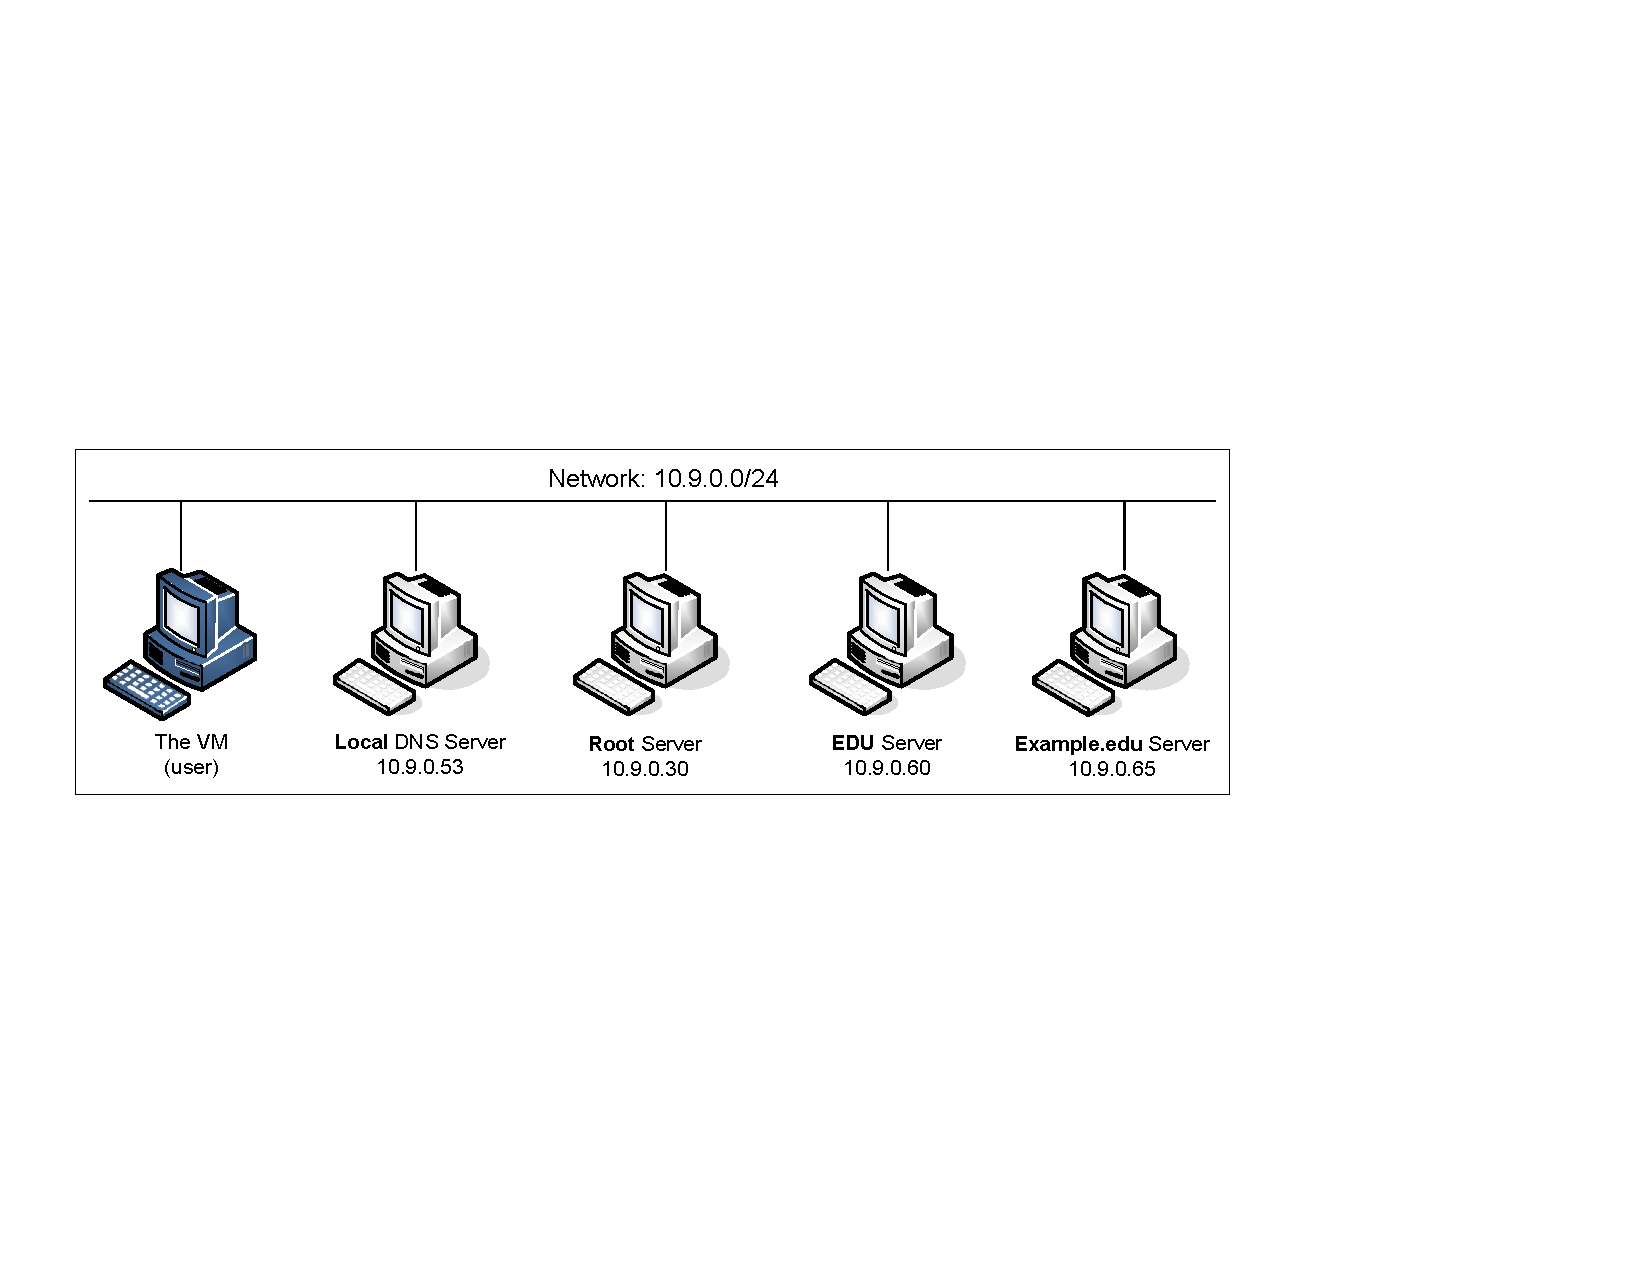
\includegraphics[width=0.95\textwidth]{Figs/DNS-in-a-box.pdf}
\end{center}
\caption{Una infraestructura de DNS simplificada}
\label{dns:fig:dns-in-a-box}
\end{figure}

En este laboratorio, construiremoss una infraestructura DNS simplificada. Empezaremos por una pequeña y gradualmente la iremos escalando.
El primer sistema DNS que haremos consistirá en cuatro nameservers, cada uno representará un rol específico en esta infraestructura DNS.
En el mundo real, estos nameservers se encuentran en redes diferentes, pero por un tema de simplicidad, en este laboratorio, los ubicaremos en la misma red.
La Figura \ref{dns:fig:dns-in-a-box} ilustra el setup del sistema.
Usaremos contenedores para correr estos nameservers.

% -------------------------------------------
% SUBSECTION
% -------------------------------------------
\subsection{Setup del Contenedor y sus Comandos}

%%%%%%%%%%%%%%%%%%%%%%%%%%%%%%%%%%%%%%%%%%%%
Para empezar a preparar el contenedor, deberá descargarse el archivo \texttt{Labsetup.zip} ubicado en el laboratorio correspondiente dentro del sitio web oficial y copiarlo dentro de la Máquina Virtual prevista por SEED. Una vez descargado deberá descomprimirlo y entrar dentro del directorio \texttt{Labsetup} donde encontrará el archivo \texttt{docker-compose.yml} que servirá para setear el entorno de laboratorio. Para una información más detallada sobre el archivo \texttt{Dockerfile} y otros archivos relacionados, puede encontrarla dentro del Manual de Usuario del laboratorio en uso, en el sitio web oficial de SEED.

Si esta es su primera experiencia haciendo el setup del laboratorio usando contenedores es recomendable que lea el manual anteriormente mencionado.

A continuación, se muestran los comandos más usados en Docker y Compose.
Debido a que estos comandos serán usados con mucha frecuencia, hemos creados un conjunto de alias para los mismos, ubicados en del archivo \texttt{.bashrc} dentro de la Máquina Virtual provista por SEED (Ubuntu 20.04)

\begin{lstlisting}
$ docker-compose build  # Build the container image
$ docker-compose up     # Start the container
$ docker-compose down   # Shut down the container

// Aliases for the Compose commands above
$ dcbuild       # Alias for: docker-compose build
$ dcup          # Alias for: docker-compose up
$ dcdown        # Alias for: docker-compose down
\end{lstlisting}


Dado que todos los contenedores estarán corriendo en un segundo plano. Necesitamos correr comandos para interactuar con los mismos, una de las operaciones fundamentales es obtener una shell en el contenedor. 
Para este propósito usaremos \texttt{"docker ps"} para encontrar el ID del contenedor deseado y ingresaremos \texttt{"docker exec"} para correr una shell en ese contenedor.
Hemos creado un alias para ello dentro del archivo \texttt{.bashrc}

\begin{lstlisting}
$ dockps        // Alias for: docker ps --format "{{.ID}}  {{.Names}}" 
$ docksh <id>   // Alias for: docker exec -it <id> /bin/bash

// The following example shows how to get a shell inside hostC
$ dockps
b1004832e275  hostA-10.9.0.5
0af4ea7a3e2e  hostB-10.9.0.6
9652715c8e0a  hostC-10.9.0.7

$ docksh 96
root@9652715c8e0a:/#  

// Note: If a docker command requires a container ID, you do not need to 
//       type the entire ID string. Typing the first few characters will 
//       be sufficient, as long as they are unique among all the containers. 
\end{lstlisting}

En caso de problemas configurando el entorno, por favor consulte la sección ``Common Problems'' en el manual ofrecido por SEED. 


%%%%%%%%%%%%%%%%%%%%%%%%%%%%%%%%%%%%%%%%%%%%



% -------------------------------------------
% SUBSECTION
% -------------------------------------------
\subsection{El archivo Docker Compose} 

Nuestro sistema DNS se compone de cuatro nameservers.
El propósito de estos cuatro nameservers se resumen a continuación:

\begin{itemize}[nosep]
\item Servidor de DNS local: realiza la resolución de nombres de otras máquinas.
\item Servidor Raíz: nameserver que sirve de zona raíz.
\item Servidor \texttt{edu}: nameserver para la zona \texttt{edu}, Top Level Domain (TLD)
\item Servidor \texttt{example.edu}: nameserver que sirve la zona \texttt{example.edu}. 
\end{itemize}

Usaremos un contenedor para cada uno de los nameservers mencionados anteriormente.
La mecánica de creación y ejecución de estos contenedores se encuentra en el archivo \texttt{docker-compose.yml}, que se incluye en el archivo de setup del laboratorio. Dentro de este archivo, hemos creado una red \texttt{10.9.0.0/24} y cuatro contenedores: cada entrada en la sección de \texttt{services} representa un contenedor. Hemos asignado una dirección IP a cada uno de los contenedores.
Observe el siguiente fragmento:


\begin{lstlisting}
services:
  seed_base_router:                       (*@\ding{80}@*)
    build: ./base_image
    image: seed-base-image-bind
    container_name: seed-base-bind
    command: " echo 'exiting ...' "

  example_edu_server:
    build:
        context: ./nameserver
        args:
            BIND_CONF_DIR: edu.example
    image: example-edu-server
    container_name: example-edu-10.9.0.65
    tty: true
    networks:
      seed-net:
        ipv4_address: 10.9.0.65

  edu_server:        ... (omitted, similar to example_edu_server) ...
        ipv4_address: 10.9.0.60
  root_server:       ... (omitted, similar to example_edu_server) ...
        ipv4_address: 10.9.0.30
  local_dns_server:  ... (omitted, similar to example_edu_server) ...
        ipv4_address: 10.9.0.53
\end{lstlisting}

En la Línea \ding{80} se especifíca la imagen base, a partir de la cual se construye la imagen base usando imagen de \path{handsonsecurity/seed-server:bind}.
Esta imagen ha sido ubicada en el Docker Hub (vea el archivo \texttt{Dockerfile} en el directorio \texttt{base\_image}).
Aunque todos los nameservers pueden generar sus contenedores basados en la imagen de Docker Hub, hemos reducido el número de accesos usados para consultar el Docker Hub (ya que la compania establece un límite en cuanto a la cantidad de accesos que un usuario en particular puede hacer durante un período de 6 horas), primero construimos una imagen local base usando la imagen de Docker Hub y después usaremos esa imagen base local para construir el resto de los contenedores del laboratorio.

% -------------------------------------------
% SUBSECTION
% -------------------------------------------
\subsection{Las Imágenes Docker} 

Exeptuando el servidor de DNS local, todos los nameservers usan el mismo directorio (\texttt{nameserver}) para construir sus imágenes. En el archivo \texttt{Dockerfile} se muestra lo siguiente:


\begin{lstlisting}
FROM seed-base-image-bind                         (*@\ding{202}@*)

ARG BIND_CONF_DIR

# Copy the BIND confirguration files
COPY named.conf named.conf.options  /etc/bind/    (*@\ding{203}@*)
COPY ${BIND_CONF_DIR}     /etc/bind/              (*@\ding{204}@*)

# Start the nameserver
CMD service named start  && tail -f /dev/null
\end{lstlisting}

La Línea \ding{202} indica que es una imagen local (que usa la imagen base).
La Línea \ding{203} copia los archivos de configuración de BIND 9 en el directorio  \texttt{/etc/bind} del contenedor. Estos archivos son los mismos para todos los nameservers, pero cada nameserver tiene su propios archivos de zona. Es por eso que se usa el argumento \texttt{BIND\_CONF\_DIR} (Línea \ding{204}) para indicar que directorio usar como el directorio por defecto de los archivos de configuración. El valor de \texttt{BIND\_CONF\_DIR} se setea en el archivo Compose.


\paragraph{Servidor de DNS local.}
La imagen del contenedor que usa el servidor de DNS local es similar a las que usan los contenedores de nameserver. Explicaremos sus diferencias más adelante, dado que la construcción de esta imagen será una de las tareas del laboratorio.


% *******************************************
% SECTION
% *******************************************
\section{Tarea l: Creando el nameserver para \texttt{example.edu}}

En esta tarea, vamos a construir un nameserver para el dominio \texttt{example.edu}. Los archivos del contenedor están dentro de la carpeta \texttt{nameserver}. 
Los archivos de configuración para este dominio en particular se encuentran dentro del subdirectorio \path{edu.example}.

\paragraph{Paso 1. Agregando la entrada de la zona}. Para hostear el dominio \texttt{example.edu} en el servidor, debemos de agregar la entrada de la zona dentro del archivo de configuración (\texttt{named.conf}) de BIND 9, de esta forma le indicamos que zona es la que va a estar hosteando. Por un tema de conveniencia agregaremos esta zona en el archivo \path{named.conf.seedlabs} que es una versión modificada del archivo \path{named.conf}.

Esta entrada indica que el nameserver actual es el servidor maestro para este dominio y su archivo de zona está especificado en la entrada dentro del archivo \texttt{file}.


\begin{lstlisting}
zone "example.edu" {
        type master;
        file "/etc/bind/example.edu.db";
};
\end{lstlisting}


\paragraph{Paso 2. Creando el archivo de la zona}. 
Al momento de construir una imagen de docker, el archivo de zona \path{example.edu.db} será copiado dentro de la carpeta \path{/etc/bind} que se encuentra en el contenedor.
Para que los estudiantes puedan empezar, hemos provisto alguna información de este archivo de zona, pero los estudiantes deberán de realizar todos los cambios que sean requeridos.

\begin{lstlisting}
$TTL 3D
@       IN      SOA   ns.example.edu. admin.example.edu. (
                2008111001
                8H
                2H
                4W
                1D)

; Records for this nameserver (you need to make changes)
@               IN   NS    ns.example.edu.
ns.example.edu  IN   A     1.2.3.4


; IP addresses for the hostnames in the example.du domain
@       IN      A     1.2.3.5
www     IN      A     1.2.3.5
xyz     IN      A     1.2.3.6
*       IN      A     1.2.3.7
\end{lstlisting}
 


\paragraph{Paso 3. Probando.} Se usará el comando \texttt{docker-compose} para generar y correr todos los contenedores. 
Una vez que los contenedores esten corriendo, ejecute el siguiente comando desde su Máquina Virtual (es decir por fuera del contenedor). Usaremos la opción  \texttt{@10.9.0.65} para enviar nuestra consulta DNS directamente a  \texttt{10.9.0.65}, que es la dirección IP del nameserver para \texttt{example.edu}. Si todo se realiza de manera correcta, obtendrá la dirección IP especificada en su archivo de zona. Por favor reporte sus observaciones.

\begin{lstlisting}
$ dig @10.9.0.65 www.example.edu
... 
;; ANSWER SECTION:
www.example.edu.    259200   IN  A   (*@\textbf{1.2.3.5}@*)
...
\end{lstlisting}



% *******************************************
% SECTION
% *******************************************
\section{Tarea 2: Creando el servidor TLD \texttt{edu}}

En esta tarea, vamos a construir un nameserver para el dominio TLD \texttt{edu}.
Modificaremos los archivos dentro de la carpeta  \texttt{nameserver/edu}.
Primero necesitamos agregar la siguiente entrada de zona en el archivo \path{named.conf.seedlabs}. Esta entrada indica que el nameserver actual es el nameserver maestro para el dominio y el archivo de zona es especificado en la entrada dentro del archivo \texttt{file}.


\begin{lstlisting}
zone "edu" {
        type master;
        file "/etc/bind/edu.db";
};
\end{lstlisting}


\paragraph{Creando el archivo de la zona.} A continuación, debemos agregar los registros en el archivo de la zona. Hemos creado el archivo de zona dentro de \texttt{edu.db}, pero está incompleto. Los estudiantes deberán de hacer los cambios necesarios.

Todos los nameservers dentro del dominio \texttt{edu} deben de registrar sus nameservers con este servidor TLD; de otra forma nadie podrá encontrarlo/resolverlo. Como ejemplo hemos agregados dos registros pra el dominio \texttt{syr.edu}: 
Un registro \texttt{NS} y un registro \texttt{A}.
El registro \texttt{NS} especifíca el nameserver para el dominio \texttt{syr.edu} mientras que el registro \texttt{A} especifíca la dirección IP del nameserver. Los datos usados en los registros son datos reales, a modo de simular que el dominio\texttt{syr.edu} ha sido registrado en nuestro servidor TLD \texttt{edu}.


\begin{lstlisting}
; Real records for syr.edu
syr.edu.                IN      NS      ns1.syr.edu.
ns1.syr.edu.            IN      A       128.230.12.8
\end{lstlisting}
 

\paragraph{Tareas.}
Los estudiantes deberán de realizar las siguientes tareas: (1) registrar el nameserver \texttt{example.edu} usando este servidor TLD; (2) elegir tres nombres de dominio reales y registrarlos dentro del servidor TLD. Puede encontrar los nameserver de un dominio usando el comando \texttt{"dig <name> NS"} (ejemplo, \texttt{"dig syr.edu NS"}).

Los estudiantes pueden usar los comandos de \texttt{docker-compose} para construir y correr todos los contenedores.
Una vez que los contenedores esten corriendo, ejecute los siguientes comandos usando \texttt{dig} desde su Máquina Virtual y envíe consultas DNS al nameserver \texttt{edu} (su dirección IP es \texttt{10.9.0.60}).
Por favor reporte sus observaciones.


\begin{lstlisting}
$ dig @10.9.0.60 www.example.edu
$ dig @10.9.0.60 www.syr.edu
$ dig @10.9.0.60 <the other three domains you have chosen>
$ dig @10.9.0.60 <a domain not included in your zone file>
\end{lstlisting}

Debe de notarse que el servidor TLD \texttt{edu} está configurado para no realizar consultas recursivas, por lo que en la consulta solamente le devolverá el nameserver para el dominio especificado; esto significa que el servidor no va a resolver la consulta por ud. 
En el último comando, ud. debería de intentar varios ejemplos con dominios (terminados en \texttt{edu}) que no están incluídos en el archivo de la zona.


% *******************************************
% SECTION
% *******************************************
\section{Tarea 4: Creando el servidor raíz}

En esta tarea, construiremos un nameserver para la zona raíz. Todos los servidores TLD necesitan registrarse con un nameserver raíz, de esta forma pueden ser encontrados en el proceso de consulta DNS.
En nuestro contenedor, la zona raíz se define dentro del archivo \texttt{bind.conf.seedlabs} que carga los registro del archivo de zona \texttt{root.db}. 

Por cada zona TLD que necesitemos agregar en nuestro sistema DNS en miniatura, necesitamos agregar al menos dos registros en el archivo de la zona, incluyendo un registro \texttt{NS} y un registro \texttt{A}. En el siguiente ejemplo, hemos agregado la información del nameserver para las zonas \texttt{com} y \texttt{net} (los datos en los registros son reales).
Esta dos zonas son manejadas por la misma compania, por lo que comparten el mismo conjunto de nameservers (hemos incluído solamente uno).

\begin{lstlisting}
com.                 IN   NS   a.gtld-servers.net.
net.                 IN   NS   a.gtld-servers.net.
a.gtld-servers.net.  IN   A    192.5.6.30
\end{lstlisting}
 

\paragraph{Tarea.} Los estudiantes deben agregar registros al archivo de la zona \texttt{root.db} que cumplan con los siguientes requerimientos:


\begin{itemize}[nosep]

\item Registre su nameserver \texttt{edu} dentro del servidor raíz.

\item Elija dos nombres de TLD reales más y regístrelos con este servidor de TLD. Uno de los TLD debe ser un TLD código de país (ccTLD), que representa la raíz de un país. Puede encontrar el nameserver de un dominio TLD usando \texttt{"dig <tld> NS"} (por ejemplo, \texttt{"dig com NS"}).
También puede encontrar toda la información relacionada a los TLD en \url{https://www.internic.net/domain/root.zone}.
\end{itemize}
 
Usando los comandos de \texttt{docker-compose}, los estudiantes pueden construir y correr todos los contenedores.
Una vez que los contenedores estén corriendo, ejecute el comando \texttt{dig} desde su Máquina Virtual y envie consultas DNS hacia el nameserver raíz (usando \texttt{"dig @10.9.0.30"}). Por favor use esta prueba para demostrar que la configuración del setup de su DNS funciona de manera correcta.


% *******************************************
% SECTION
% *******************************************
\section{Tarea 5: Creando el servidor de DNS local} 

Cuando una máquina necesita resolver una dirección IP de un hostname (o visce versa), envía una consulta a un "ayudante" denominado servidor de DNS local (no necesita ser local en realidad). Este servidor de DNS local será el encargado de manejar el proceso de resolución y enviar el resultado de regreso hacia la máquina que hizo la consulta.
En esta tarea, haremos el setup para este servidor de DNS local.


\paragraph{Root hint file.}
Si el servidor de DNS local no puede encontrar la respuesta dentro de su caché, este entrará en un proceso iterativo para encontrar la respuesta en los nameservers externos a este. El proceso comienza desde el servidor raíz.
Además, el servidor de DNS local necesita saber la dirección IP de los servidores raíz.

Dentro de \path{/etc/bind/named.conf.default-zones}, que está incluído en el archivo de configuración de \bind (\path{/etc/bind/named.conf}), existe una entrada para cada zona raíz. Esta entrada especifíca un archivo de sugerencia (hint file) para cada zona raíz, de esta forma el servidor de DNS local tiene conocimiento de la dirección IP de cada servidor raíz.


\begin{lstlisting}
zone "." {
	type hint;
	file "/usr/share/dns/root.hints";
};
\end{lstlisting}

El archivo raíz de sugerencia (root hint file) especifíca los nameservers para cada zona raíz (existen 13 nameservers para la zona raíz). La dirección IP (v4 y v6) para cada uno de estos nameservers se encuentran dentro de este archivo.
El siguiente ejemplo muestra un fragmento del archivo.

\begin{lstlisting}
.                        3600000      NS    A.ROOT-SERVERS.NET.
A.ROOT-SERVERS.NET.      3600000      A     198.41.0.4
A.ROOT-SERVERS.NET.      3600000      AAAA  2001:503:ba3e::2:30
...
\end{lstlisting}

Dentro del directorio \texttt{local\_dns\_server} de los archivos de setup del laboratorio, hemos creado un archivo vacío llamado \texttt{root.hints}. Este archivo será copiado dentro de la carpeta \path{/usr/share/dns/} al momento de crear el contenedor del servidor de DNS local.
Ud. necesitará agregar esos registros dentro de este archivo, así su servidor de DNS local puede usar su servidor raíz en vez de usar los que pertenecen al mundo real.


\paragraph{Probando.} Use los comandos de \texttt{docker-compose} para construir y correr todos los contenedores.
Una vez que los contenedores estén corriendo ejecute el siguiente comando desde su Máquina Virtual, \texttt{"dig @10.9.0.53"} este comando enviará consultas DNS al servidor de DNS local (su dirección IP es  \texttt{10.9.0.53}).
Por favor reporte sus observaciones.

\begin{lstlisting}
$ dig @10.9.0.53 www.example.edu
$ dig @10.9.0.53 www.example.com
$ dig @10.9.0.53 www.example.net
$ dig @10.9.0.53 www.syr.edu
$ dig @10.9.0.53 www.xyz.<TLD registered with your root server>
$ dig @10.9.0.53 www.xyz.<TLD not registered with your root server>
\end{lstlisting}



% *******************************************
% SECTION
% *******************************************
\section{Tarea 6: Configurar nuestra Máquina Virtual para usar el servidor de DNS local} 

Hast ahora, usamos \texttt{@<ip>} en conjunto con el comando \texttt{dig} para indicar cual es el servidor DNS que debe de contactar el comando \texttt{dig}. Mientras que esto no es un problema para \texttt{dig}, es un problema para otro tipos de programas que dependen del servicio de DNS. Necesitamos indicarle al sistema operativo que el contenedor del servidor de DNS que vamos a generar en esta tarea, será el servidor de DNS local por defecto que va a usar el sistema.

Esto se logra cambiando el archivo de configuración (\texttt{/etc/resolv.conf}) en la máquina del usuario de manera tal que se agregará la dirección IP del contenedor como la primera entrada \texttt{nameserver} dentro de este archivo, es decir, este servidor será usado como el servidor de DNS primario.
Desafortunadamente nuestra Máquina Virtual usa DHCP para obtener los parámetros de la configuración de red, tales como la dirección IP, el servidor de DNS local, etc. Los clientes DHCP sobreescribirán el archivo \texttt{/etc/resolv.conf} con su la información provista por el servidor DHCP.

Una forma de evitar esto es agregar la siguiente entrada dentro del archivo \path{/etc/resolvconf/resolv.conf.d/head}:

\begin{lstlisting}
Add the following entry to /etc/resolvconf/resolv.conf.d/head
  nameserver 10.9.0.53

Run the following command for the change to take effect
$ sudo resolvconf -u
\end{lstlisting}

El contenido del archivo head será antepuesto al que se usa en la generación dinámica por el DHCP.

Después de haber terminado la configuración en la máquina del usuario, repita la prueba del testeo de los comandos que ejecutados en la Tarea 5, pero esta vez no incluya \texttt{@<ip>} en los comandos. Preste atención a las direcciones IP remarcardas para asegurarse que la respuesta provienen de su contenedor. Si la configuración no se hizo de manera correcta, la dirección IP será diferente.

\begin{lstlisting}
$ dig abc.example.edu

...
;; ANSWER SECTION:
abc.example.edu.	259200	IN	A	1.2.3.7

;; Query time: 3 msec
;; SERVER: (*@\textbf{10.9.0.53}@*)#53(10.9.0.53)
...
\end{lstlisting}
 

\paragraph{\ding{72}\ding{72} Nota (Muy importante) \ding{72}\ding{72}.} 
Una vez terminado el laboratorio, recuerde borrar la entrada agregada en \path{/etc/resolvconf/resolv.conf.d/head}; si esto no se hace, pueden ocurrir muchos problemas en futuros laboratorios. Si en un futuro, ud. tiene problemas para conectarse a Internet, pero su red se encuentra funcionando, existen probabilidades de que ud. haya olvidado borrar esta entrada y esto estropeará el proceso de consultas DNS. Esto me ha ocurrido varias veces y frecuentemente olvido borrar esta entrada. 


% *******************************************
% SECTION
% ******************************************* 
\section{Tarea 7: Haciéndolo mas Real}

En esta tarea, haremos que nuestro sistema DNS en miniatura sea un poco más realista agregando los siguientes nameservers o registros a nuestro sistema.


\begin{itemize}
\item Agregue 2 o más servidores raíz. En el mundo real el sistema DNS tiene 13 direcciones IP para cada servidor raíz. En este laboratorio crearemos 3.

\item Seleccione dos TLDs registrados en su servidor raíz, construya un dominio de segundo nivel para cada uno de ellos, use su apellido como nombre de dominio.
Por ejemplo, si su apellido es \texttt{Smith}, necesita crear los nameservers para los dominios \texttt{smith.<tld1>} y \texttt{smith.<tld2>}.
Necesita hostear ambos dominios en el mismo nameserver.
\end{itemize}




%Note: try to avoid using \texttt{com} and \texttt{net}. It 
%is harder, because they depend on each other.

 


% *******************************************
% SECTION
% ******************************************* 
\section{Informe del Laboratorio}

%%%%%%%%%%%%%%%%%%%%%%%%%%%%%%%%%%%%%%%%

Debe enviar un informe de laboratorio detallado, con capturas de pantalla, para describir lo que ha hecho y lo que ha observado.
También debe proporcionar una explicación a las observaciones que sean interesantes o sorprendentes.
Enumere también los fragmentos de código más importantes seguidos de una explicación. No recibirán créditos aquellos fragmentos de códigos que no sean explicados.
%%%%%%%%%%%%%%%%%%%%%%%%%%%%%%%%%%%%%%%%

\paragraph{Limpieza.} Este es un recordatorio en el que se avisa nuevamente que se debe de borrar la entrada añadida en \path{/etc/resolvconf/resolv.conf.d/head}.

% *******************************************
% SECTION
% *******************************************
\section*{Agradecimientos}

Este documento ha sido traducido al Español por Facundo Fontana



\end{document}
